\chapter{Introduction}
\label{cha:intro}

%\section{Spatial cognition and probability}
%\label{sec:intro:brainspaceprob}

Brains have evolved to move bodies through space in order to increase the chances of survival and reproduction, through numerous complex behaviours such as fleeing from threats or searching for nutrients or potential mates. The ability to remember spatial information, e.g. previously encountered food sources or shelters, has provided sufficient evolutionary advantage that all known organisms with brains (and even some without, such as the slime mold\footnote{Slime molds are able to avoid previously explored areas using externalized spatial memories, and to solve mazes using nutrient gradients} - \citet{reid2012slime}) have at least a rudimentary ability to utilize representations of space for more efficient navigation. Higher mammals have evolved a network of brain areas implementing spatial memory, a system for storing and recalling spatial information about the environment and about their location in it.

Representing spatial information accurately in the real world is hard, for several reasons. Sensors and actuators are limited, erroneous and noisy (in the sense of noise interfering with the signal). There are additional sources of uncertainty or unknown information, such as external events, actions of other organisms, unperceived or currently unperceivable objects or events. Furthermore, physical environments can be highly complex, and yet cognitive resources (amount of memory, processing power, time and energy available) are necessarily limited by biological and physical constraints. 

In artificial intelligence (AI) and robotics research, probabilistic models have provided key tools for dealing with such challenges, facilitating the quantitative characterization of beliefs and uncertainty in the form of probability distributions, and the machinery of Bayesian inference for updating them with new data. They have also inspired the `Bayesian brain' \citep{knill2004bayesian} and `Bayesian cognition' \citep{chater2010bayesian} paradigms in the cognitive sciences. These paradigms have been successful in explaining human behaviour in tasks as diverse as the integration of sensory cues \citep{ernst2006bayesian} including spatial information \citep{cheng2007bayesian,nardini2008development}, sensorimotor learning \citep{kording2004bayesian}, visual perception \citep{yuille2006vision} or reasoning \citep{oaksford2007bayesian}. Their success suggests an answer to what biological cognition might be doing to cope with the above-mentioned challenges: approximate Bayesian inference.

\begin{figure}[h]
	\centering
	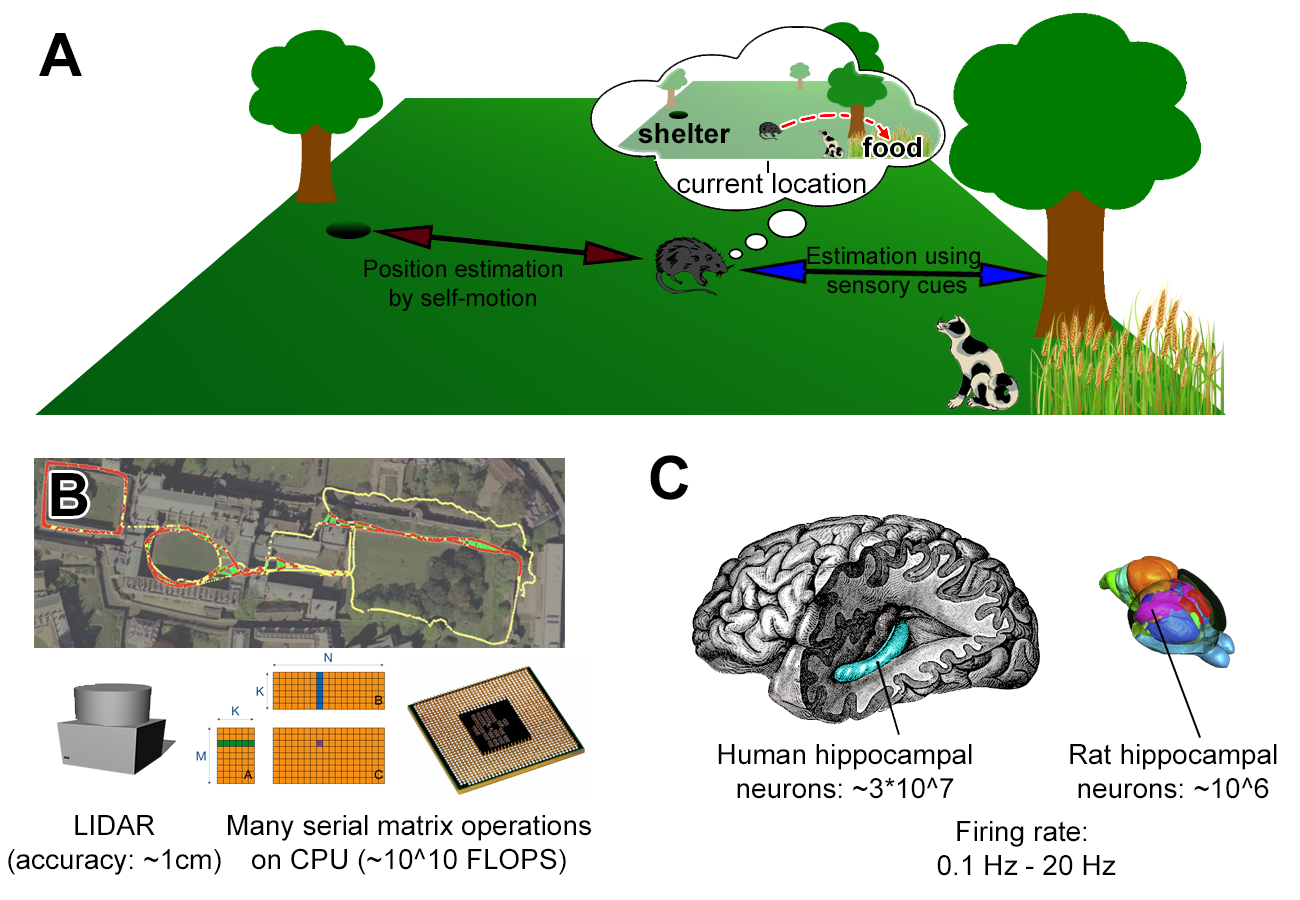
\includegraphics[width=\textwidth]{img/motivation}
	\caption[Motivation for proposing new computational cognitive models of spatial memory]{\textbf{Motivation for proposing new computational cognitive models of spatial memory}. A: Learning representations of the space around animals confers significant advantages, such as the ability to plan a detour out of sight (dashed red arrow) to reach a food source while avoiding danger in this example. In real environments, this task is made more difficult by the unreliability, errors and noise inherent in both the estimation of position by integrating self-motion and in estimated object distances (e.g. based on vision). Most existing cognitive models of spatial memory neglect these challenges. B: State of the art SLAM models in robotics are able to estimate locations and learn maps accurately, but rely on sensors and computations which are very different from biology - e.g. higher measurement accuracy using laser-based distance sensors (LIDAR), centralized control and coordination, and high number of serial operations per second - up to $10^{10}$ floating-point operations per second (FLOPS) needed for state of the art SLAM systems \citep{machado2013evaluation}. C: In contrast, the hippocampus - the major brain area involved in world-centered spatial representations - contains only a few million neurons, of which only a subset is active at a time, each firing only a few times per second \citep{rapp1996preserved,vsimic1997volume}; and relies on noisy, inaccurate sensory measurements. Although many models of spatial memory in brains exist, there is a lack of computational mechanisms which are both neurally and psychologically plausible, and can work in realistic environments and with noisy sensors. (Example SLAM data in Panel B from \citep{newman2011describing}, and 3D rat brain in Panel C from \citep{calabrese2013ontology}, with permission.)} 
	\label{fig:motivation}
\end{figure}

\section{Motivation}
\label{sec:intro:motivation}

Despite of this success and of the suitability of probabilistic models to deal with uncertain and noisy spatial information, there have been few attempts to use them for modelling spatial memory within cognitive modelling, the branch of cognitive science concerned with computationally simulating mental processes. There is a gap in the literature between probabilistic spatial models in robotics and computational cognitive models of spatial memory. In robotics, Simultaneous Localization and Mapping (SLAM) models \citep{thrun2008simultaneous} are capable of dealing with real-world noise, uncertainty, and complexity to some extent, but are cognitively implausible\footnote{In our usage of the terms, a computational model is `psychologically plausible' (or `cognitively plausible') to the extent that it is consistent with psychological findings and can accurately reproduce psychology data, i.e. behaviours. Analogously, it is `biologically plausible' (or `neurally plausible') to the extent that it is consistent with neuroscience and can reproduce neural data, e.g. single-cell recordings or brain imaging results.}. On the other hand,  current computational cognitive models of spatial memory, which are designed to model biological spatial cognition,  cannot deal with all of these challenges, and are thus confined to simplistic simulations (see Chapter \ref{cha:nnreview} for a review, and Figre \ref{fig:motivation} for an overview of the importance of spatial memory and the differences between information processing in robots and brains). 

%There is also a dearth of models of \textit{how} neurons could be able to perform Bayesian inference to improve spatial representations, and of evidence on a neuronal level (as opposed to behavioural) that they can. 

In addition, although spatial representations in humans have been argued early to be hierarchical \citep{hirtle1985evidence, mcnamara1989subjective, greenauer2010micro}, similarly to some robotic implementations having to deal with large, complex environments \citep{kuipers2000spatial, wurm2010octomap}, it is not known how (by which process) these hierarchical spatial maps might be structured. Although many computational models of spatial memory running in simplified environments exist, there is a lack of biologically and psychologically plausible `algorithms' serving as models of human cognitive computations related to spatial information processing which can 

\clearpage

\noindent function in realistic, uncertain, complex environments.

The deprioritization of the problems of uncertainty and noise in favour of tractably modelling other human cognitive mechanisms is also pronounced in cognitive architectures, which try to account for a large number of mental processes in a unified, comprehensive, systems-level model (as opposed to computational cognitive models, which usually focus on a single phenomenon). In their overview of the field, \cite{langley2009cognitive} argue that \textit{`` we should attempt to unify many findings into a single theoretical framework, then proceed to test and refine that theory''}, supporting the arguments of \cite{newell1973you} that \textit{``you can't play 20 questions with nature and win''}, highlighting the importance of systems-level research in the cognitive sciences. Although a few such cognitive architectures do model spatial mechanisms in navigation space \citep{harrison2003act,schultheis2011casimir,sun2004top}, they all run in simple, noise-free environments. According to a comparative table of cognitive architectures \citep{samsonovich2011comparative} available in updated form online\footnote{http://bicasociety.org/cogarch/architectures.htm}, there is currently no cognitive architecture implementing both Bayesian update and an empirically validated, psychologically plausible `cognitive map' at the same time.
%\footnote{CogPrime \citep{goertzel2013cogprime} claims to implement both Bayesian update and cognitive maps, but neither of these mechanisms have been evaluated against human data, or indeed claim to be modelling human cognitive phenomena at all. Instead, CogPrime aims for artificial general intelligence, as opposed to closely adhering to human cognition.}.

The present work was motivated by these gaps in the literature, and aims to take computational cognitive models of navigation-scale\footnote{Human cognition needs to keep track of the space of navigation as well as the spaces immediately around the body (e.g. reachable objects) and of the body (e.g. body-part configurations). Although uncertainty and noise play are important in the latter two spaces as well, we will confine ourselves to navigation-scale spatial mechanisms in this work.} spatial memory one step closer to modelling behaviour in realistic environments, such as high-fidelity robotic simulations or physical environments. It aims to do so by means of proposing probabilistic mechanisms of spatial cognition which are implementable in brains and can reproduce behaviour data, and by computationally implementing these mechanisms, in the form of cognitive models and within an existing cognitive architecture. Situated within the computational sub-fields of cognitive science (cognitive modelling and cognitive architectures), the goal of this work is to contribute to the understanding of information processing in human cognition. As such, although it is computational in nature, the extent of its success is determined by its ability to predict and explain the kinds of behaviour data it is intended to model, as well as its consistency with established findings in psychology and neuroscience. It is not aiming to maximize the accuracy of learned spatial representations, unlike robotics. Neither does it aim for neurobiological fidelity at the cellular level or below. Although building on neuroscientific evidence, our concern is modelling spatial information processing on Marr's algorithmic level of analysis \citep{marr1976understanding, marr1977understanding}, as opposed to e.g. biological neural networks - see Table \ref{tbl:marr} -, with Chapter \ref{cha:bayespc} being the single exception. 

\begin{table*}[h]
	\centering
	{\renewcommand{\arraystretch}{1.2}
		\begin{tabu}{c|c|c}
			$\downarrow$ {Level of analysis} & {Description} & {In this work}\\ \tabucline[3pt]{-}
			1. Computational & \begin{tabular}[c]{@{}c@{}} What problem(s) does the \\ system solve, and why? \end{tabular} & \begin{tabular}[c]{@{}c@{}} Localization,\\ Map error correction, \\ Map structuring \end{tabular} \\\hline
			\begin{tabular}[c]{@{}c@{}} \textbf{2. Algorithmic/} \\ \textbf{Representational} \end{tabular} & \begin{tabular}[c]{@{}c@{}} How might it solve them? (Using\\ what representations and processes?) \end{tabular} & \begin{tabular}[c]{@{}c@{}} Cognitive models \\ of spatial memory \end{tabular} \\\hline
			3. Implementation & How is it implemented physically? & \begin{tabular}[c]{@{}c@{}} Place, grid,  head- \\ direction, border cells, \\ ... \citep{hartley2014space} \end{tabular} \\
		\end{tabu}
	}
	\caption[Investigating spatial mechanisms on Marr's (1976) levels of analysis]{\textbf{Investigating spatial mechanisms on Marr's (1976) levels of analysis}. The present work is mostly concerned with the second level.}
	\label{tbl:marr}
\end{table*}
%\begin{tabular}[c]{@{}c@{}} Approximately Bayes- \\optimal integration\\of information \end{tabular}

% Although this mechanism has been empirically substantiated on a behavioural level before \citep{cheng2007bayesian, nardini2008development}, its

We have investigated the plausibility of Bayesian spatial cue integration both on Marr's algorithmic (Chapter \ref{cha:lida}) and implementation level (Chapter \ref{cha:bayespc}), in order to maintain the desirable criteria of both psychological and neural plausibility for our other models. The possible neural implementation of this mechanism has been unknown, with current mechanistic models of Bayesian inference in brains making assumptions not fully consistent with the anatomy or activity of the hippocampal complex (the major brain areas representing world-centered spatial information) - see next Section. This doubt of biological implementability has motivated our investigation of single-cell electrophysiological data (acquired outside this PhD) to provide the first evidence for Bayesian updating in the hippocampus on a neuronal level, and our proposal of a plausible mechanism for implementing it. This evidence, presented in Chapter \ref{cha:bayespc}, affords a degree of biological plausibility to the models utilizing Bayesian mechanisms in the rest of our work (which is concerned with processes on the algorithmic/representational level).

%especially if behavioural evidence is inconclusive or insufficient to constrain the space of possible models to a concrete implementation

\section{Probabilistic models of space in brains and minds}
\label{sec:intro:uncertaintybrain} 

Although the focus of most of this work is on the computational modelling of behaviour data, we would like the employed mechanisms to be plausibly implementable in the parts of the brain they functionally correspond to. Apart from the lack of neuronal-level evidence that the hippocampal complex may perform Bayesian inference or even represent uncertainty, the possibility of the implementation of such a mechanism given the anatomical and electrophysiological constraints of this network of brain cells is also unclear. 

Below, we briefly review probabilistic neural spatial models which have been proposed in the literature (Chapter \ref{cha:nnreview} provides a more general review of computational cognitive models of spatial memory). We start with normative models of dealing with spatial uncertainty, which derive optimal solutions to the problem a system might be solving (Marr's computational level). We then continue describing mechanistic (implementation level) models which might facilitate these, and their consistency with what is known about the hippocampal complex. More extensive reviews of Bayesian models in brains can be found in \citep{pouget2013probabilistic, vilares2011bayesian}. There is currently little experimental support for any of the proposed neural uncertainty representations. % \citep{pouget2013probabilistic}. 

%In addition to a large number of non-probabilistic computational cognitive models focusing on accounting for specific mechanisms of spatial cognition (see Chapter \ref{cha:nnreview} for a review), a few authors have suggested probabilistic mechanisms the brain might employ which can be used to model spatial cognition.

Models of probabilistic estimation of spatial information have been pioneered by \citep{bousquet1997hippocampus}, who suggested to use a Kalman filter to model localization in the hippocampus. A Kalman filter is a dynamic Bayesian inference algorithm for estimating the values of unknown, not directly observable variables (such as location) from noisy observations, yielding statistically optimal estimates if the noise is normally distributed \citep{kalman1960new}. \citet{macneilage2008computational} also put forth arguments for dynamic Bayesian inference as a model of spatial orientation. They mention both Kalman filters and particle filtering (a related Bayesian filtering algorithm using samples instead of parameters to represent probability distributions), but leave the question of their neural implementation open. Particle filter-based models of localization on the algorithmic level have been suggested by \citep{fox2010hippocampus, cheung2012maintaining}. \citet{osborn2010kalman} went beyond localization, suggesting a Kalman filtering approach to also account for localizing objects in the environment. Recently, \citet{penny2013forward} argued that if one presupposes the existence of `observation' and `dynamic' models\footnote{Observation models and dynamic models are mathematical functions mapping from true states to observed states, and from pre-motion to post-motion states, respectively.}, required by Kalman filters, one might as well extend the inference to also use them for model selection (`which environment am I in?'), motor planning (`how do I get to place X?'), and to construct sensory imagery (`what does place X look like?') in addition to localization. They have combined these functions in a single probabilistic model, and argued that it is consistent with findings of pattern replay in the brain. An even more general probabilistic formulation based on dynamic Bayesian inference is the Free-Energy Principle \citep{friston2006free}, which aspires to provide a unified theory of brain function, and has been argued to be consistent with aspects of hippocampal processing \citep{friston2011action}.

Despite their considerable theoretical elegance, the above-mentioned models do not provide a final and complete answer to the motivating question of this thesis (Section \ref{sec:intro:motivation}), which can be summarized as: `how does biological cognition learn representations of navigation space from noisy sensors in an uncertain world?', for two reasons. First, none of them try to reproduce or show quantitative consistence with either behavioural or neural data concerning spatial cognition (although qualitative consistence with anatomical and neural findings is pointed out by the authors). Although these models provide explanations, their predictions regarding spatial processing have not been quantitatively evaluated.

Second, in addition to the lack of quantitative validation, their neural implementation is not known, and far from straightforward. For example, implementing the kinds of large matrix inversions and multiplications required by Kalman filters \citep{kalman1960new} is easy on a computer, with centrally coordinated, serial, `fast' computations, but difficult with the kind of distributed, parallel, `slow' (on the level of single neurons, which only spike up to a few dozen times per second) computation performed by the brain. In the domain of world-centered, navigation-scale spatial mechanisms, any suggested neural implementation has to conform with not only the limitations imposed by biological neural networks, but also with the specific connectivity and activity observed in the hippocampal complex, in order to be considered biologically plausible.

In addition to such normative models, a number of mechanistic (implementation-level) models of how uncertainty and inference could be implemented in brains have also been proposed. They can be roughly grouped into three categories - see \citep{pouget2013probabilistic, vilares2011bayesian} for reviews. We briefly summarize these groups below, together with their consistency with what is known about the hippocampus. 
%, which would be suitable for spatial localization or map learning in the face of uncertainty, together with the main reason we chose not to adopt that mechanism in this work. Detailed arguments regarding these reasons can be found in Appendix A.

% free-form approximations do not scale

% no electrophysiological or psychophysical evidence to suggest that the brain can encode multimodal approximations:

\begin{itemize}

\item Probabilistic population codes (PPC) \citep{ma2006bayesian} encode probability distributions in the logarithmic domain by means of a set of coefficients of corresponding exponential basis functions, each coefficient encoded by the activity (spike count) of a neuron. They assume neural variability is independent and Poisson-distributed. However, hippocampal neurons exhibit more variability than a Poisson process \citep{fenton1998place, barbieri2001construction}. Also, if Bayesian inference were implemented in the hippocampus via a PPC, the encoded probability distributions would strongly depend on the firing rate of hippocampal neurons: increased firing rates should mean decreased levels of uncertainty. But empirically, this is not the case - for example, firing rates increase with movement speed \citep{maurer2005self}, which would mean the lowest uncertainties when running fastest (however, faster movements are harder to control and should thus lead to higher uncertainty). 

\item Instead of an encoding in the logarithmic domain, codes in which firing rates are proportional to probabilities have also been proposed, e.g. by \citet{koechlin1999bayesian, barber2003neural}. The problem with their implementation in hippocampal neurons is that the firing rates of these neurons are also influenced by factors unrelated to probability, such as where the animal is headed \citep{ferbinteanu2003prospective} or trial dependent features \citep{allen2012hippocampal}, and can change substantially if either the shape or colour of an environment is altered \citep{leutgeb2005independent}. These influences would strongly interfere with the outcome of the Bayesian inference, if it were implemented in a code that directly utilizes firing rates.

\item Sampling-based codes represent probability distributions with a set of samples drawn from them \citep{fiser2010statistically}. They are asymptotically correct with infinitely many samples, and approximations otherwise. Apart from being able to represent complex, multi-modal distributions, not having to rely on any fixed-form parametrization such as Gaussians, this also allows reducing their accuracy and computational demands by restricting the number of samples used. This property has been used e.g. by \citep{shi2010exemplar} to explain the deviations from the statistical optimum in an exemplar model of a reproduction task. It is difficult to make a general statement as to the implementability of this class of models in the hippocampal complex, as there is a wide variety of suggested concrete neural implementations in non-spatial domains (\citet{sanborn2015types} provides a review), and some applied to navigation space, e.g. \citep{fox2010hippocampus, cheung2012maintaining}. None of them have been quantitatively validated by neural (electrophysiological) measurements, although most of them are supported by behavioural observations. 

%\item \citet{deneve2007optimal} [attractor networks] %  rather than coding for the log probability that a feature is present, neurons code for the log probability that a feature takes on a particular value
%\item \citet{ma2006bayesian} [PPC]
%\item \citet{fiser2010statistically} [sampling]
%\item \citet{friston2011action} [FEP]

\end{itemize}

How the brain might encode and utilize uncertainty is still an open question \citep{pouget2013probabilistic}, but based on the observations regarding the hippocampus outlined above, we argue that a sampling-based code is most suitable in this brain area; in terms of violating as few empirical observations as possible. We will provide electrophysiological evidence of Bayesian inference from single neurons, and propose a possible sampling-based mechanism, in Chapter \ref{cha:bayespc} (and in more detail in Appendix \ref{apx:bayespc}).


%bousquet et al kalman filter

%fox prescott

%penny pioneered ... extend this line of research... difficult to actually implement, as EKF O(n^2)

%Khamassi and Humphries [18] argue that, due to the shared underlying neuroanatomy, spatial navigation strategies that were previously described as being either place-driven or cue- driven are better thought of as being model-based versus model- free. Daw et al. [15] propose that arbitration between model-based and model-free controllers is based on the relative uncertainty of the decisions

% friston action understanding

% make things as simple as possible, but not simpler

% implicitly - RatSLAM

\section{Hypotheses}
\label{sec:intro:hypotheses}

To achieve goals in a spatially extended, realistic environment, at a minimum, an agent (e.g. a biological agent such as an animal, or an artificial agent such as a robot) must be able to 1) move, and keep track of its movements, 2) sense, and interpret its sensations, 3) represent spatial locations in its environment, e.g. of itself and its goal, 4) update these representations when changes occur in the environment, and 5) utilize these representations to achieve its goals (e.g. navigate to its goal location, avoiding dangers). Extensive work on all levels of analysis has been carried out for 1)-3), with the most recent Nobel prize in physiology or medicine awarded on the topic of 3) to John O'Keefe, May-Britt Moser and Edvard I Moser for the discovery of \textit{`cells that constitute a positioning system in the brain'} \citep{burgess2014nobel}. Specifically, it was awarded for the discovery of `place cells' in the hippocampus (which show increased firing in a specific area in the environment, called its `place field'), and of `grid cells' which show a regular, grid-like firing pattern (see Chapter \ref{cha:nnreview} below). 

We have argued above that despite of the variety of existing models regarding 4)+5), new computational models are needed to move towards biological and psychological plausibility as well as real-world capability at the same time (since biological cognition has been shaped by the constraints and challenges of the real world, these should not be neglected in models of cognition). In particular, in accordance with the `Bayesian brain' \citep{knill2004bayesian} and `Bayesian cognition' \citep{chater2010bayesian} paradigms, we have suggested approximate Bayesian inference to be a well-suited mechanism for tackling these challenges. Models on Marr's algorithmic (and implementation) level which utilize such a mechanism require a number of underlying assumptions, some of which can be stated and evaluated as hypotheses. 

We summarize major hypotheses in one place in Table \ref{tbl:hyp} below, and expand on them in the respective results chapters below. The first two concern the representation and manipulation of uncertainty in the hippocampus (required for maintaining approximately accurate location estimates despite noisy sensors and accumulating errors). Hypothesis 3 is needed since unless all remembered landmark locations are corrected at every moment (which would likely be intractable), a discrepancy between remembered and actual locations might arise when revisiting a location encountered previously (when traversing a `loop' in the environment). This discrepancy necessitates a backward correction of multiple recent self and landmark locations to maintain consistent representations. The last two are needed to formulate a computational mechanism of spatial representation structure. Structured, hierarchical representations provide clear computational advantages, such as increased speed and efficiency of retrieval search, and economical storage. However, although strong neural \citep{derdikman2010manifold} and behavioural \citep{hirtle1985evidence, mcnamara1989subjective, greenauer2010micro} evidence exists for such structure, underlying computational principles have remained largely unknown.

\newpage

\setlength\tabcolsep{4pt}
%\small
\begin{longtable}{|p{4.5cm}|p{4.5cm}|p{4.6cm}|}
	\hline
	\textbf{Hypothesis} & \textbf{Prediction} & \textbf{Empirical support} \\
	\hline
	
	1 Hippocampal place cells can perform approximate Bayesian inference & {Place field size depends on uncertainty (e.g. proximity of landmarks) in a} & {Place field sizes (recorded from hippocampal neurons of behaving rats) are cor-} \\ \cline{1-1} 
	2 Spatial uncertainty is represented as the size of place cell firing fields & Bayesian fashion & related with uncertainties predicted by a Bayesian model (Chapter \ref{cha:bayespc}) \\ \hline
	3 When revisiting a place, estimates of recently traversed locations and encountered landmarks are updated in an approx. Bayes-optimal fashion & After revisiting parts of an environment, place fields should shift, and recently active place cells should re-activate. Errors should conform to Bayesian predictions & Neural: none in this work, but place fields seem to shift after revisits \citep{mehta2000experience}, and recently active place cells do reactivate (`replay') \citep{carr2011hippocampal}. Behavioural: errors correlate with predictions (Chapter \ref{cha:lida}) \\ \hline 
	4 The structure of spatial representations arises from clustering & Landmarks which are co-represented (belong together) in participants' & Neural: none in this work. Behavioural: the probability of two landmarks being \\ \cline{1-1}
	5 This clustering mechanism operates on features including Euclidean distance, path distance, boundaries, visual and functional similarity & spatial memory should be closer in these features than those not belonging together & co-represented is strongly correlated with distances along these specific features. These distances allow prediction of participant representation structure (Chapter \ref{cha:structure}) \\
	
	\hline
	\captionsetup{width=\textwidth}
	\caption[Hypotheses of the models presented in this work]{\textbf{Hypotheses of the models presented in this work, and empirical support}. Place cell electrophysiological recording data was acquired outside this PhD. All other data has been collected by the author, unless otherwise specified.}
	\label{tbl:hyp}
\end{longtable}


\section{Outline and Contributions}
\label{sec:intro:outline}

This thesis is presented in the Alternative Format allowed by the University of Manchester presentation of theses policy \footnote{http://documents.manchester.ac.uk/DocuInfo.aspx?DocID=7420}, which allows incorporating sections in a format suitable for publication in peer-reviewed journals. We chose the alternative format to more easily accommodate already published work, to reduce risks of self-plagiarism,  and because of the largely self-contained nature of our individual results chapters. Thus, in what follows, the literature review (Chapter \ref{cha:nnreview}) and the three chapters (\ref{cha:bayespc}-\ref{cha:lida}) reporting the results, are copies of papers either accepted by or submitted to peer-reviewed journals. The following list summarizes these papers and the contributions\footnote{In all publications, Madl wrote the draft of the paper, developed the software, designed the experiments, recruited and tested the participants where applicable, and analysed the data. Corrections suggested by Chen, Montaldi, and Franklin were incorporated into the final drafts by Madl after discussions with these co-authors. All publications were supervised by Chen and Montaldi, with Chen mainly commenting on mathematical and computational issues, and Montaldi on psychological and neuroscientific issues.} therein:

\begin{itemize}
	\item Chapter \ref{cha:nnreview}: Madl T., Chen K., Montaldi D. \& Trappl R., 2015. Computational cognitive models of spatial memory in navigation space: A review. \textit{Neural Networks, 65, 18-43.}
	\\ Contributions: 1) a systematic review of representative cognitive models concerned with navigation-scale spatial memory, falling into symbolic, neural network, or cognitive architecture models, including a comparative table of the characteristics of these models.
	\item Chapter \ref{cha:bayespc}: Madl T., Franklin S., Chen K., Montaldi D. \& Trappl R., 2014. Bayesian Integration of Information in Hippocampal Place Cells. \textit{PLoS ONE 9(3), e89762}
	\\ Contributions: 2) first quantitative electrophysiological validation of the representation of spatial uncertainty in the brain, and of Bayesian integration of spatial information in the brain, in three different environments (using data acquired outside this PhD). 3) Formulation and empirical support for an inference mechanism based on coincidence detection (falling into the camp of sampling-based models of neural inference)
	\item Chapter \ref{cha:structure}: Madl T., Franklin S., Chen K., Trappl R. \& Montaldi D., submitted. Exploring the structure of spatial representations. \textit{Cognitive Processing}
	\\ Contributions: 4) behavioural evidence for clustering as the normative principle underlying spatial representation structure, and 5) the first computational model of navigation-scale spatial representation structure on the individual level (able to predict this structure in participants' long-term spatial memory from the geospatial properties of an environment)
	\item Chapter \ref{cha:lida}: Madl T, Franklin S, Chen K, Montaldi D \& Trappl R, submitted. Towards real-world capable spatial memory in the LIDA\footnote{LIDA stands for Learning Intelligent Distribution Agent, and is reviewed in a paper co-authored during this PhD but not included in this thesis: \citep{franklin2013lida}} cognitive architecture. \textit{Biologically Inspired Cognitive Architectures}
	\\ Contributions: 6) integration of three spatial mechanisms capable of dealing with uncertainty and noise into a comprehensive cognitive architecture (localization, map structuring, map correction), and 7) embodying this architecture on a robot, allowing demonstration of the model functionality in a realistic robotic simulator. 8) Proposal of a biologically plausible mechanism for correcting errors in learned maps when revisiting an already known place (the `loop closure' problem, well known in robotics, but neglected in cognitive science), and evaluation against behaviour data regarding cognitive map accuracy in human subjects.
\end{itemize}

The model best accounting for spatial memory structure presented in Chapter \ref{cha:structure} also constitutes a novel kind of metric learning in machine learning, based on the idea of learning a similarity function in the space of absolute pairwise differences (as opposed to e.g. a Mahalanobis distance function). Although proposed before in a similar form for person re-identification in the computer vision community \citep{zheng2011person}, the insight that this space contains neglected information which can be utilized to improve performance in general (not just on image data), and the general formulation allowing arbitrary constituent models for learning a metric in this space, are a novel contribution (9). Since it is too far from the topic of this thesis, metric learning in absolute pairwise difference space is only described briefly (to the extent required to model cognitive map structure) in Chapter \ref{cha:structure}. Applications and results on other kinds of data, with other constituent models, and in a semi-supervised setting, and are briefly summarized in Appendix \ref{apx:adsmetric}.

Before presenting the mentioned papers constituting the literature review and results chapters, we briefly overview the computational methods employed during this research in Chapter \ref{cha:methods} (they are also described in the respective results chapters). After the computational methods, we present the literature review (Chapter \ref{cha:nnreview}) and results (Chapter \ref{cha:bayespc}-\ref{cha:lida}) in the form of published or submitted papers. Subsequently, we continue to discuss the implications of our results, the neural implementability of these mechanisms, and the shortcomings and limitations of our models in Chapter \ref{cha:discussion}. We conclude in Chapter \ref{cha:conclusion} with a conclusion and an outline of potential future work opened up by this research. 

We note that the line of criticism mentioned regarding the neural implementability of the high-level probabilistic models of localization in the previous section also apply to our proposed mechanism of cognitive map structuring (Chapter \ref{cha:structure}). Although it is intended to be a cognitive and not a neural model, we have argued that consistency with the underlying neuroscience can and should play a role in constraining the space of possible models, and evaluating models, even on the algorithmic level. But the map structuring mechanism in Chapter \ref{cha:structure} is, to our knowledge, the first formal model of the observed structure in cognitive maps, both on Marr's computational and algorithmic levels. We did not have the time and resources to extend it down to include a plausible neural implementation within this PhD.

Finally, work done during this PhD has contributed to two more publications which are not included in this thesis (the former because it is a conference paper, whereas University policy requires alternative format theses to contain journal papers instead; and the latter because it does not fit in well with the main topic):


%
%\begin{itemize}
%	\item Madl T., Franklin S., Chen K. \& Trappl R., 2013. Spatial working memory in the LIDA cognitive architecture. \textit{Proceedings of the International Conference on Cognitive Modelling (2013), pp. 384-389}
%	\item Franklin S., Madl T., D'Mello, S., Snaider, J., 2014. LIDA: A Systems-level Architecture for Cognition, Emotion, and Learning. \textit{IEEE Transactions on Autonomous Mental Development 6(1), pp. 19-41}
%\end{itemize}